\documentclass[a4paper,12pt]{article}
\usepackage{graphicx}
\usepackage{booktabs}
\usepackage{geometry}
\usepackage{amsmath}
\usepackage{float}

\geometry{top=2cm, bottom=2cm, left=3cm, right=2cm}

\begin{document}

\begin{titlepage}
    \centering
    \vspace*{1cm}
    
    {\LARGE \bfseries Department of Information and Communication Technology \par}
    \begin{figure}
        \centering
        \includegraphics[width=1\linewidth]{logo-number.jpg}
    \end{figure}
    
    \vspace{2cm}
    
    {\Huge \bfseries Machine Learning in Medicine \par}
    
    \vspace{1cm}
    
    {\Large ECG Heartbeat Classification Report \par}
    
    \vfill
    
    \begin{minipage}{0.5\textwidth}
        \begin{flushleft}
            {\large \textbf{ID - Student Name:}} \\
            22BI13103 - Le Duc Dung - Data Science
        \end{flushleft}
    \end{minipage}%
    \begin{minipage}{0.5\textwidth}
        \begin{flushright}
            {\large \textbf{Lecturer:}} \\
            Prof. Tran Giang Son
        \end{flushright}
    \end{minipage}
    
    \vspace{2cm}
    
    {\large Academic year: 2022 - 2025} \par
    
    \vspace{1cm}
    
    {\large Hanoi, February 2025}
    
\end{titlepage}

\section{Introduction}
This report presents Practical 1 of Machine Learning in Medicine, where a publicly available Kaggle dataset is analyzed to understand its structure and features before developing a classification model. The study involves a detailed description of the dataset, including its features, sources, and preprocessing steps. A machine learning approach is implemented to build a classification model such as the Support Vector Machine and its performance is thoroughly evaluated. The results are then compared with those reported in the original research paper to assess the effectiveness of the proposed model.

\section{Dataset}
The MIT-BIH Arrhythmia Dataset is a widely used benchmark for ECG classification tasks. It contains 187 features that describe heartbeat signals recorded at a 125 Hz sampling rate. The dataset categorizes heartbeats into five classes.. Normal, Atrial Premature, Premature Ventricular Contraction, Fusion of Ventricular and Normal, and Paced beats. It consists of 87,554 training samples and 21,892 testing samples but suffers from a class imbalance, with the Normal class being the most prevalent.

\subsection{Arrhythmia Dataset}
\begin{itemize}
    \item \textbf{Number of Samples:} 109,446
    \item \textbf{Number of Categories:} 5
    \item \textbf{Sampling Frequency:} 125Hz
    \item \textbf{Data Source:} Physionet's MIT-BIH Arrhythmia Dataset
    \item \textbf{Classes:} 
    \begin{itemize}
        \item \textbf{N}: 0
        \item \textbf{S}: 1
        \item \textbf{V}: 2
        \item \textbf{F}: 3
        \item \textbf{Q}: 4
    \end{itemize}
\end{itemize}

\subsection{The PTB Diagnostic ECG Database}
\begin{itemize}
    \item \textbf{Number of Samples:} 14,552
    \item \textbf{Number of Categories:} 2
    \item \textbf{Sampling Frequency:} 125Hz
    \item \textbf{Data Source:} Physionet's PTB Diagnostic Database
\end{itemize}

\subsection{Class Distribution}
This dataset suffers from class imbalance with Normal class taking the highest distribution among others on both train-set and test-set.

\begin{figure}
    \centering
    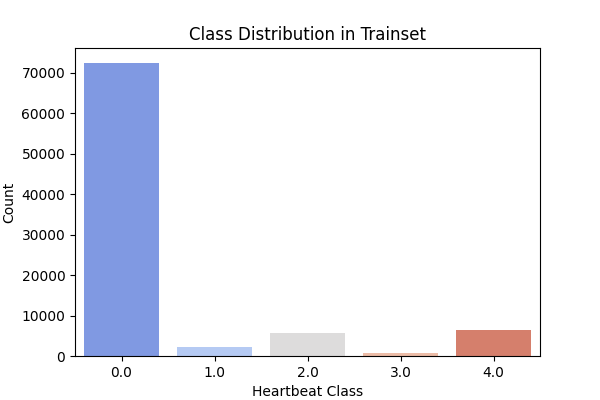
\includegraphics[width=1\linewidth]{figures/Trainset_label_distribution.png}
    \caption{Train-set Label Distribution}
    \label{fig:enter-label}
\end{figure}
\begin{figure}
    \centering
    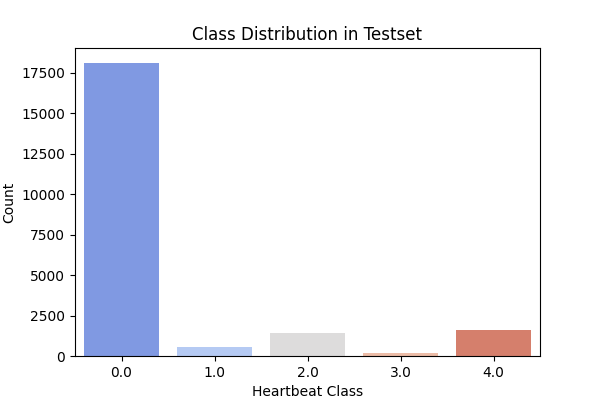
\includegraphics[width=1\linewidth]{figures/Testset_label_distribution.png}
    \caption{Test-set Label Distribution}
    \label{fig:enter-label}
\end{figure}

\section{Methodology}
This section is about how the Support Vector Machine is trained with the preprocessed dataset.

\subsection{Preprocessing}
Since the training dataset is imbalanced, we use SMOTE (Synthetic Minority Over-sampling Technique) from Imblearn Library to resample the class distribution for achieving better results.

\begin{equation}
    x_{\text{new}} = x_{\text{current}} + \lambda \times (x_{\text{neighbor}} - x_{\text{current}})
\end{equation}

where \( \lambda \) is a random number between 0 and 1.

\subsection{Model Architecture}

Support Vector Machine is a machine learning model with low computational-cost. And SVC (Support Vector Classification) is particularly effective for high-dimensional datasets and cases where decision boundaries are complex.

\vspace{0.5cm}

Given a training dataset \( (x_i, y_i) \), where:

\begin{itemize}
    \item \( x_i \) is a feature vector,
    \item \( y_i \in \{-1,1\} \) represents class labels,
\end{itemize}

The goal is to find a hyperplane:

\begin{equation}
    w \cdot x + b = 0
\end{equation}

where \( w \) is the weight vector and \( b \) is the bias.

The margin is maximized by solving:

\begin{equation}
    \min_{w,b} \frac{1}{2} \|w\|^2
\end{equation}

subject to:

\begin{equation}
    y_i (w \cdot x_i + b) \geq 1, \quad \forall i
\end{equation}

\begin{table}[H]
    \centering
    \begin{tabular}{lcccc}
        \toprule
        Param & Value \\
        \midrule
        C & 1.0 \\
        break\_ties & False \\
        cache\_size & 200 \\
        class\_weight & None \\
        coef0 & 0.0 \\
        decision\_function\_shape & ovr \\
        degree & 3 \\
        gamma & scale \\
        kernel & rbf \\
        max\_iter & -1 \\
        probability & False \\
        random\_state & None \\
        shrinking & True \\
        tol & 0.001 \\
        verbose & False \\
        \bottomrule
    \end{tabular}
    \caption{SVC Hyperparameters}
    \label{tab:svc_params}
\end{table}

\section{Results}

This section will show the classification report and confusion matrix of SVC model on test dataset.

\begin{table}[H]
    \centering
    \begin{tabular}{lcccc}
        \toprule
        Class & Precision & Recall & F1-score & Support \\
        \midrule
        0 & 0.97 & 1.00 & 0.98 & 18,118 \\
        1 & 0.96 & 0.56 & 0.71 & 556 \\
        2 & 0.97 & 0.86 & 0.91 & 1,448 \\
        3 & 0.76 & 0.46 & 0.57 & 162 \\
        4 & 1.00 & 0.90 & 0.95 & 1,608 \\
        \midrule
        Accuracy &  &  & 0.97 & 21,892 \\
        Macro Avg & 0.93 & 0.76 & 0.82 & 21,892 \\
        Weighted Avg & 0.97 & 0.97 & 0.96 & 21,892 \\
        \bottomrule
    \end{tabular}
    \caption{Classification Report}
    \label{tab:classification}
\end{table}

The proposed model outperforms the previous benchmark in all key metrics. It achieves a precision of 97\%, significantly higher than the prior 95. 9\%, demonstrating an improved overall performance. Its 98\% precision surpasses 95.2\%, indicating better positive prediction reliability. Furthermore, its 98\% recall exceeds 95.1\%, showing improved sensitivity in detecting all classes. These enhancements suggest better class balance handling and machine learning algorithms that can handle data imbalance.

\begin{figure}[H]
    \centering
    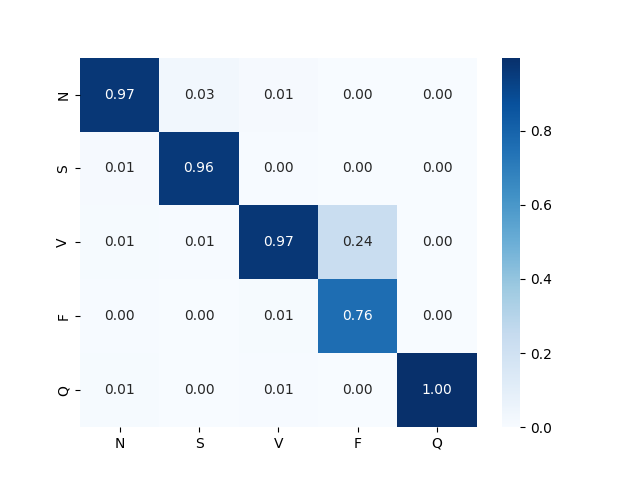
\includegraphics[width=1\linewidth]{figures/Confusion_Matrix_applying_SMOTE.png}
    \caption{Confusion Matrix}
    \label{fig:enter-label}
\end{figure}

The confusion matrix has strong diagonal elements in class N(97\%), S(96\%), V(97\%), Q(100\%) which indicates that the SVC model performs quite well in distinguishing these classes. However, there are some overlapping characteristics (class V has 24\% misclassification rate into class F) due to the imbalance in train dataset. 

\end{document}
